\documentclass[]{auvsi_doc}
\setkeys{auvsi_doc.cls}{
	AUVSITitle={Autopilot and Path Planner Requirements Matrix},
	AUVSIRevision=.1,
	AUVSIDescription={Initial Draft},
	AUVSIAuthor={Brady Moon},
	AUVSIChecker={John Akagi},
	AUVSILogoPath={./figs/logo.pdf},
	AUVSIDocID={RM-002}
}

% include extra packages, if needed
\usepackage[skip=-50pt]{caption}

% Remove Heading Numbers
\setcounter{secnumdepth}{0}

% Remove Heading Numbers
\setcounter{secnumdepth}{0}

\begin{document}
\begin{AUVSITitlePage}
\begin{artifacttable}
	\entry{CT-005, 0.1, 02-28-2019, Initial requirements,Brady Moon, John Akagi}
	\entry{CT-005, 1.0, 02-28-2019, Requirements matrix added,John Akagi, Andrew Torgesen}
	\entry{CT-005, 1.1, 04-05-2019, Market Response Added, John Akagi, Andrew Torgesen}
\end{artifacttable}
\end{AUVSITitlePage}
% document contents

\section{Introduction}
This artifact describes the requirements matrix for the autopilot subsystem (See Figure \ref{fig:reqMat}). The measured values are taken from the five simulated tests and one hardware test which are described in CT-003, Path Planner Testing Procedures and Results. The market response is based on the competition rules where ``Impressive" indicates more than 90\% of the points would be obtained, ``Good" indicates that more than 80\% of the points would be obtained, ``Fair" indicates that more than 70\% of the points would be obtained, and ``Poor" indicates that less than 70\% of the points would be obtained. Values which are important to the efficiency or efficacy of the system but are not directly evaluated during the competition are marked with ``N/A".

%\begin{figure}
	\begin{center}
	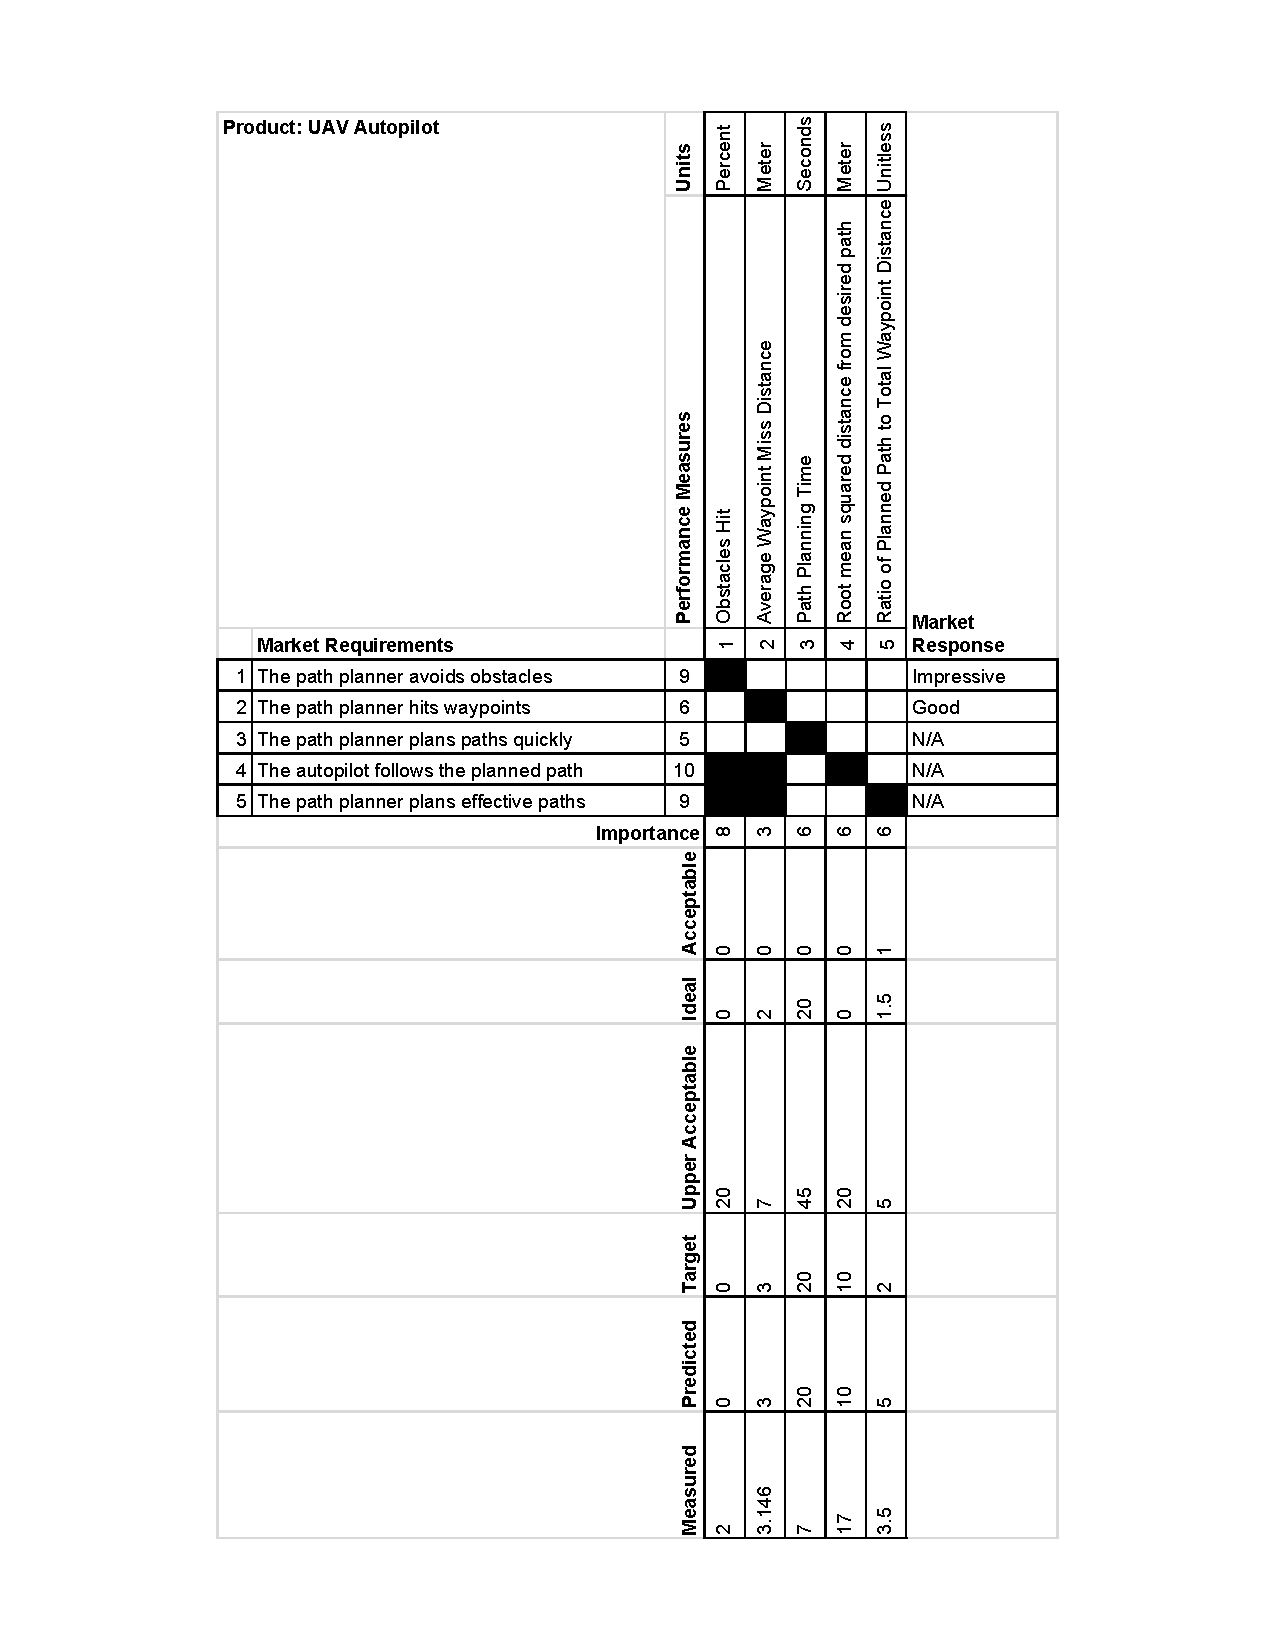
\includegraphics[width=0.6\textwidth]{./figs/RequirementsMatrix.pdf}
	\vspace{2cm}
	\captionof{figure}{Requirements matrix for the subsystem which will control the UAV.}
	\label{fig:reqMat}
	\end{center}

	% \AUVSIFigure
	% {./figs/RequirementsMatrix.pdf}
	% {0.55\textwidth}
	% {Requirements matrix for the subsystem which will control the UAS.}
	% {fig:reqMat}
%\end{figure}

\end{document}
